\documentclass[11pt]{article}
\usepackage[a4paper,margin=2.5cm]{geometry}
\usepackage{setspace}
\onehalfspacing
\usepackage[T1]{fontenc}
\usepackage{lmodern}
\usepackage[natbibapa]{apacite}
\renewcommand{\doiprefix}{https://doi.org/}
\usepackage{amsmath,amssymb,amsthm,booktabs,graphicx,xcolor,algorithm,algpseudocode}
\usepackage[hidelinks]{hyperref}
\graphicspath{{figures/}}
\newtheorem{theorem}{Theorem}
\newtheorem{proposition}[theorem]{Proposition}
\newtheorem{corollary}[theorem]{Corollary}
\newtheorem{lemma}[theorem]{Lemma}
\theoremstyle{definition}
\newtheorem{definition}[theorem]{Definition}
\newtheorem{example}[theorem]{Example}
\newcommand{\E}{\mathbb{E}}
\newcommand{\Prob}{\mathbb{P}}
\newcommand{\lord}{\ell_\lambda}

\begin{document}
\begin{titlepage}
\begin{center}
{\Large\bfseries Fair vehicle routing with random route durations:\\[2pt]
ex-post ordered fairness, rank prices and risk-consistent tours\par}
\vspace{1.5em}
{\large Quang-Vinh Dang\textsuperscript{a,}\footnote{Corresponding author. E-mail address: \texttt{vinh.dq4@buv.edu.vn} (Q.-V.~Dang). ORCID: 0000-0002-3877-8024.},
Hoang-Viet Vu\textsuperscript{a},
Phuc-Son Nguyen\textsuperscript{b}\par}
\vspace{1em}
{\small
\textsuperscript{a}School of Computing, British University Vietnam, Hung Yen, Vietnam\\
\textsuperscript{b}School of Economic Mathematics -- Statistics, University of Economics Ho Chi Minh City, Ho Chi Minh City, Vietnam\par}
\end{center}
\vspace{2em}
\noindent E-mail addresses: \texttt{vinh.dq4@buv.edu.vn} (Q.-V.~Dang), \texttt{30066017@st.buv.edu.vn} (H.-V.~Vu), \texttt{sonnp.3393@ueh.edu.vn} (P.-S.~Nguyen).
\end{titlepage}

\begin{abstract}
Fair vehicle routing minimises an ordered measure of route lengths, such as
the range or the Gini mean difference, and recent exact approaches require
every route to be a shortest tour of its customers. They assume deterministic
travel times, whereas drivers experience realised durations. We study fair routing
with random travel times and distinguish ex-ante fairness, of expected
workloads, from ex-post fairness, the expected unfairness of the realised
day. We prove that deterministic fair plans overstate ex-post fairness, bound
the gap, and show that it is largest for balanced plans. We give an exact, sampling-free integral for the expected value of any
ordered measure of independent route durations, based on the
Poisson--binomial distribution, and derive rank prices, the derivatives of
expected unfairness with respect to each route. Because even the minimax
objective can prefer a longer tour under uncertainty, we define route
consistency through each driver's mean and standard deviation and show that
the consistent tours are supported Pareto tours. A bilevel local search uses the rank prices to screen moves. In seventeen
experiments on two families of benchmark instances, deterministic fair plans
understate realised unfairness by 8 to 40 percent. Optimising ex-post fairness
improves realised fairness by about 1 percent at the standard budget, 2
percent on a second instance family (better on all twelve instances)
and up to 7 percent with generous budgets, while using less of the
budget. It outperforms sample average approximation and a risk-adjusted
baseline that is no better than ignoring uncertainty.
\end{abstract}

\noindent\textbf{Keywords:} Routing; Fairness; Stochastic travel times; Order statistics; Bilevel optimization


\section{Introduction}

Routing plans that minimise total distance often give some drivers much
longer days than others. Unequal workloads hurt driver satisfaction and
retention and can be seen as unfair \citep{matl2018workload}. The fairness
literature in routing therefore optimises a \emph{fairness measure} of the
vector of route workloads: the longest route, the range, the Gini mean
difference (GMD), the variance or a mean absolute deviation
\citep{matl2018workload,karsu2015inequity,bektas2020lp}. Ordered measures, which
weight the sorted workloads \citep{yager1988owa,ogryczak2003solving,nickel2005location},
cover all of these in one framework \citep{blanco2026optimization}.

Non-monotone measures such as the range or the GMD create a well-known
pathology: an optimiser can lower the measure by making a light route
\emph{longer}, giving a driver a needless detour
\citep{matl2018workload}. \citet{vanrossum2026efficient,vanrossum2026enforcing}
and \citet{ljubic2026fair} close this loophole exactly, by requiring every route to
be a shortest tour of its customers, i.e.\ an optimal solution of the
travelling salesman problem (TSP) on its customers. \citet{ljubic2026fair}
write the problem as a bilevel programme in which a planner assigns customers
and each driver solves a TSP, and solve instances with up to 35 customers to
optimality for seven measures.

All of these works assume deterministic travel times. A driver's day,
however, is a realised duration: congestion, weather, parking and
service-time variability differ between routes and between days. Fairness
is then a statement about random variables, and three questions arise that
the deterministic theory does not ask.
\begin{enumerate}
\item \emph{What should be balanced?} The expected workloads (ex-ante
fairness), or the workloads drivers actually experience, sorted day by day
(ex-post fairness)? The identity of the worst-off driver changes from day to
day, and the two notions can disagree.
\item \emph{How can ex-post fairness be optimised?} Sample-average
approximation (SAA) is the default, but sorting per scenario makes the
objective noisy and its gradient uninformative.
\item \emph{What is a consistent route?} Under random durations "the
shortest tour" is not obviously what a driver would choose, and we show
that monotone measures no longer protect drivers from detours.
\end{enumerate}

\paragraph{Contributions.}
\begin{itemize}
\item \textbf{Model.} We formulate fair routing with random travel times
(a fleet-wide day factor times arc-level noise) as a bilevel problem with an
ex-post ordered fairness objective, an expected-cost budget and per-driver
risk-consistent tours. With no noise it reduces to the fair capacitated vehicle routing problem with
shortest-tour routes (X-CVRP-TSP) of \citet{ljubic2026fair}.
\item \textbf{Fairness illusion (Proposition~\ref{prop:gap}).} For every
ordered measure with nondecreasing weights, ex-ante fairness underestimates
ex-post unfairness, by at most $\|\lambda\|_1 v (\sum_k W_k)^{1/2}$, where
$W_k$ is the route's quadratic length. Common multiplicative shocks leave the
expected value of every ordered measure unchanged
(Proposition~\ref{prop:common}); they do inflate the variance measure and the
tail of unfairness.
\item \textbf{Poisson--binomial order-statistic integral (PBOI;
Theorem~\ref{thm:pboi}).} An exact, sampling-free formula for
the expected ordered measure of independent route durations with given
marginals (we use moment-matched gamma marginals), as an integral
of a Poisson--binomial distribution against tail sums of the weights. It
handles negative weights and costs $O(Gm^2)$.
\item \textbf{Rank prices (Proposition~\ref{prop:prices}).} The derivative of expected
unfairness with respect to a location shift of a route's duration equals the
expected weight of its rank. Prices of dispersion measures sum to zero, and a negative price is
precisely the stochastic incentive to lengthen a route.
\item \textbf{Risk-consistent tours (Proposition~\ref{prop:mono}, Theorem~\ref{thm:supported}).}
Even $\E\max$ can prefer a non-shortest tour. We define consistency through the
driver's own mean--standard deviation and prove that the consistent tour is a
supported Pareto tour of (length, quadratic length), found exactly by
dichotomic parametric Held--Karp.
\item \textbf{Algorithm and evidence.} SORTIE (Stochastic Ordered Route
fairness with Tour-consistency via Integral Evaluation), a bilevel local
search whose
moves are screened by rank prices, is compared with the deterministic fair plan,
SAA with up to 5000 scenarios, a risk-adjusted deterministic baseline and
ablations, in seventeen experiments: on the instances used by the
deterministic literature and on a second family of twelve CVRPLIB instances,
with exact enumeration on small instances, budget, fleet-size, noise-level
and risk-attitude sweeps, four noise models including correlated noise, and
up to 100 customers.
\end{itemize}

%==========================================================================
\section{Literature review}\label{sec:lit}

SORTIE sits at the intersection of four literatures: workload equity in
deterministic vehicle routing, inequity-averse optimisation with ordered
measures, fairness under uncertainty, and routing with stochastic travel
times. We review each in turn, stating for the closest works what they model,
how they solve it and what they leave open, and close with the tools we
borrow from probability and multicriteria optimisation.
Table~\ref{tab:positioning} summarises the positioning.

\subsection{Workload equity in deterministic routing}

The systematic study of balanced routing starts with
\citet{matl2018workload}, who compare the equity functions used in the
literature (min-max, range, mean absolute deviation, Gini-type
measures and others) on the same instances. Their central observation is
that the measures differ in \emph{monotonicity}: a measure that is not
monotone in the individual workloads can be improved by making a short route
longer, so an optimal ``fair'' plan may contain routes that are needlessly
inefficient. \citet{matl2019impact} show that the choice of the workload
resource (distance, duration, load or number of customers) changes the
balanced plan and the cost of equity, and
\citet{matl2019leveraging} approximate the cost--balance Pareto front with a
box-splitting scheme around a single-objective heuristic. In all three works
the workload is a deterministic quantity attached to a route.

Exact methods have followed two directions. The min-max (makespan) objective
has a long tradition \citep{applegate2002solution}, and
\citet{bertazzi2015minmax} quantify how much longer the longest route can
become when total cost is minimised instead. For balance objectives,
\citet{halvorsen2016biobjective} study bi-objective general routing with
several balance criteria, \citet{bektas2020lp} propose $\ell_p$ norms
of the workload vector as a tunable family between efficiency and min-max
fairness, and \citet{agius2026solution} develop exact algorithms for routing
with route-cost equity \emph{constraints}. \citet{vanrossum2024branching,vanrossum2026efficient}
design branching rules for range and order-based objectives that make the
range tractable in branch-and-price, and \citet{vanrossum2026enforcing} add
cutting planes that forbid arc sequences dominated by a shorter tour of the
same customers, which removes exactly the inefficiency identified by
\citet{matl2018workload}. Related models balance tours in the multiple
travelling salesman problem with a bound on the Gini coefficient of tour
lengths \citep{bhadoriya2026equitable}, trade egalitarian against
utilitarian welfare in cooperative fleets \citep{lopezsanchez2024fair},
weigh the cost of driver satisfaction \citep{bruinink2025beyond}, equalise
\emph{cumulative} workload across periods by assigning daily routes to drivers
\citep{nekooghadirli2026workload}, and allocate workload among heterogeneous drivers by Nash social welfare under a
cost cap \citep{mahmoodian2025equitable}, and design equity-oriented workload
and pay for crowdsourced drivers \citep{sobhanan2026equity}.

The direct predecessor of this paper is \citet{ljubic2026fair}. They write a
whole family of fairness objectives (maximum, range, Gini mean difference,
absolute deviation, variance) as ordered measures of the vector of route
lengths, borrowing the ordered-median machinery of location theory, and
resolve the monotonicity problem of \citet{matl2018workload} with a
\emph{bilevel} formulation: the upper level chooses the partition of the
customers, and each lower level must route its customers on a shortest tour.
They solve the resulting X-CVRP-TSP exactly on instances sliced from CVRPLIB
X-n641-k35, which we reuse. Their model, like every work in this subsection,
is deterministic; their conclusion lists uncertain demands as future work
and does not discuss travel-time uncertainty. SORTIE keeps their bilevel
structure and their ordered measures but lets route durations be random.
Three things change. The objective becomes an expectation of an ordered
measure of random variables, which no deterministic formulation represents
(Section~\ref{sec:theory}). Monotonicity no longer guarantees that the
optimal tours are shortest ones (Proposition~\ref{prop:mono}), so route
consistency must be imposed for every measure, not only for the
non-monotone ones. And ``shortest'' itself needs a definition when the
duration of a tour is a random variable; we give one through each driver's
mean--standard-deviation criterion and show that it is computable
(Theorem~\ref{thm:supported}).

\subsection{Ordered measures and inequity-averse optimisation}

Ordered weighted averaging was introduced by \citet{yager1988owa} as an
aggregation that weights outcomes by their rank rather than by their
identity; with nondecreasing weights it is convex and contains the maximum,
the range and the Gini mean difference as special cases. In location theory
the same idea became the ordered median problem
\citep{nickel2005location}, with linear programming representations of
sorted sums through top-$k$ sums \citep{ogryczak2003minimizing,ogryczak2003solving}
and a theory of equitable location built on inequality measures
\citep{ogryczak2000inequality}. Recent work extends the machinery to equity
within facilities \citep{blanco2024intra}, to Benders decomposition for the
discrete ordered median problem \citep{ljubic2024benders}, to quadratic
ordered measures such as the variance \citep{blanco2026optimization}, and to
the ordered median travelling salesman problem, in which the edges of a
single tour are weighted by rank \citep{ljubic2026ordered}. The broader
inequity-averse literature is surveyed by \citet{karsu2015inequity}, and
\citet{tsang2026unified} characterise a class of convex fairness measures and
show how stable optimal solutions are with respect to the choice of measure.
In all of these works the ordered measure is applied to a deterministic
vector. Our Theorem~\ref{thm:pboi} gives the expectation of an ordered
measure of independent random variables in closed integral form, and
Proposition~\ref{prop:prices} its derivative with respect to each component;
we are not aware of an analogue in the ordered-median literature.

\subsection{Fairness under uncertainty}

Only a handful of papers combine routing, fairness and uncertainty, and none
of them concerns the fairness of drivers' random workloads.
\citet{kinable2026fair} study a stochastic vehicle routing problem with
partial deliveries in which demand is random and fairness is defined among
\emph{customers}, as a minimum expected fill rate with a Rawlsian criterion;
the quantity to be shared is the service received, not the work done. \citet{gao2026sequential} combine sequential fair allocation with
routing under demand uncertainty and define max-min objectives over
locations, both ex post (per realisation) and in a forward sense; again the
recipients of fairness are locations, and the measure is max-min rather
than a general ordered measure. On the workforce side, \citet{anh2022workload}
assign tasks to workers with uncertain service times so that the difference
in total working time stays below a threshold with high probability, using a
distributionally robust joint chance constraint approximated by the worst-case
conditional value-at-risk (CVaR); there is no routing. \citet{lin2022robust} design two-echelon routes
for meal delivery with a workload-fairness criterion among workers and
protect it against service-time uncertainty with robust constraints; the
fairness measure is evaluated on the deterministic side of the robust
counterpart, not as a distribution of realised workloads. Gig-economy and
rideshare work treats fairness of assignment \emph{probabilities} and of
matching under stochastic arrivals \citep{singh2023fairassign,nanda2020balancing}
and fair allocation of delivery tasks \citep{basik2021fair,hosseini2025algorithmic};
the object is an assignment, not the duration of a route.

The word \emph{consistency} is used differently in the consistent vehicle
routing problem, where it means that customers are visited by the same driver
at similar times across days \citep{groer2009consistent,kovacs2015generalized}.
This notion has been extended to stochastic customers and demands with a
two-stage model solved by sample average approximation and decomposition
\citep{alvarez2024consistent}, to robust demand \citep{wu2025exact} and to
driver equity with flexible consistency \citep{yu2024consistent}. It is
unrelated to the route consistency of \citet{ljubic2026fair} and of this
paper, which requires each route to be an optimal tour of its own customers.

The distinction between ex-ante and ex-post fairness that organises our model
is well established outside routing. In welfare economics,
\citet{fleurbaey2012exante} contrast equality of prospects with equality of
outcomes. \citet{gutjahr2021inequity} formalises ex-ante and ex-post
inequity aversion in stochastic decision processes and relates them to
time consistency, and \citet{mostajabdaveh2019inequity} combine ex-ante and
ex-post Gini-based inequity in stochastic shelter location, followed by
\citet{alem2022revisiting} for two-stage humanitarian location--allocation and
by \citet{mostajabdaveh2025branch} for a bi-objective relief routing problem
with a Gini index of unsatisfied demand. \citet{sinclair2023sequential}
characterise the envy--efficiency trade-off of sequential allocation under
stochastic demand, \citet{shehadeh2023reducing} reduce disparities in
transport distance in stochastic facility location,
\citet{ye2024distributionally} define distributional fairness through
Wasserstein distances, and \citet{barak2026exante} use exactly our two
definitions (the measure of expected loads against the expected measure) in
facility-location mechanism design. These works establish that the two
notions differ and that the ex-post one is the relevant one for affected
individuals; none of them concerns routing or ordered measures of random
route durations. We bring the distinction to fair routing, quantify the gap
between the two notions (Proposition~\ref{prop:gap}) and show how to optimise
the ex-post notion exactly in the objective.

\subsection{Stochastic travel times in vehicle routing}

Routing with random travel times has a rich literature, but its objectives
are cost, feasibility or reliability rather than equity.
\citet{laporte1992vehicle} introduce a priori routes with chance-constrained
and recourse models, \citet{kenyon2003stochastic} include a makespan-type
objective on the expected or quantile completion time of the longest route,
and \citet{bakach2021solving} study makespan objectives with correlated
travel times; these are the closest to our maximum measure, but they
optimise a moment or quantile of the makespan, not an ordered measure of all
routes, and they do not consider the dispersion of workloads. Distribution
fitting and correlation are discussed by \citet{gomez2016modeling},
stochastic and robust formulations with deadlines by
\citet{adulyasak2016models}, a priori optimisation with recourse for time
windows by \citet{errico2016apriori,errico2018vehicle}, the cost--service
trade-off by \citet{zhang2013stochastic}, service-level guarantees by
\citet{ehmke2015ensuring}, and CVaR-type risk in latency location-routing by
\citet{osoriomora2025riskaverse}; the surveys of \citet{oyola2018part1} and
\citet{gendreau2016future} give the wider picture. Correlated travel times are
handled exactly by \citet{rostami2021branch} and approximately by
\citet{rajabibahaabadi2021reliable,bomboi2022stochastic}; robust and
distributionally robust variants include \citet{han2014robust},
\citet{jaillet2016routing}, \citet{zhang2021distribution} and
\citet{ghosal2020distributionally}. Sample average approximation
\citep{verweij2003sample} is the generic alternative to our closed-form
evaluation, and we compare against it directly (E15). Mean--risk path choice
\citep{sen2001meanvariance,nikolova2014meanrisk} motivates our definition of
a risk-consistent tour as one that minimises the driver's mean plus a
multiple of the standard deviation. Conditional value-at-risk
\citep{rockafellar2000optimization,rockafellar2002conditional}, which we report
for the realised range, and the price of fairness
\citep{bertsimas2011price,mo2000fair}, which E9 traces for stochastic
fairness, complete the background.

\subsection{Order statistics and parametric optimisation}

Our evaluator rests on classical results on order statistics of independent,
non-identically distributed variables. Their joint distribution can be
written with permanents \citep{vaughan1972permanent,bapat1989order}, which
are expensive to evaluate \citep{balakrishnan2007permanents,glueck2008fast};
the alternative we use expresses the event ``at most $r$ variables lie below
$t$'' through the Poisson--binomial distribution of the number of successes
in independent non-identical trials \citep{hoeffding1956distribution}, whose
probability mass function is computed exactly by a short recursion
\citep{fernandez2010closed,hong2013computing,biscarri2018simple}; see also
\citet{david2003order} and \citet{sen1970note}. To our knowledge the
Poisson--binomial representation has not been used to evaluate or
differentiate ordered fairness measures in optimisation. For the lower level,
supported efficient solutions of bi-criteria problems are enumerated by
dichotomic (weighted-sum) search \citep{aneja1979bicriteria}, see
\citet{ehrgott2005multicriteria,ehrgott2000survey,ralphs2006improved}, and
small travelling salesman problems are solved by the Held--Karp recursion
\citep{heldkarp1962dynamic,bellman1962dynamic}.

\begin{table}[t]\centering\small
\caption{Positioning of SORTIE among the closest works. Drivers: fairness
among drivers' workloads; Ordered: general ordered measures; Random
durations: route durations are random; Ex post: fairness of realised
outcomes is optimised; Consistency: every route is an optimal tour of its
customers. ($\circ$: partly, see text.)}\label{tab:positioning}
\setlength{\tabcolsep}{4pt}
\resizebox{\textwidth}{!}{\begin{tabular}{lcccccc}
\toprule
Work & Routing & Drivers & Ordered & Random durations & Ex post & Consistency\\
\midrule
\citet{matl2018workload} & \checkmark & \checkmark & $\circ$ & & & \\
\citet{vanrossum2026enforcing} & \checkmark & \checkmark & $\circ$ & & & \checkmark \\
\citet{ljubic2026fair} & \checkmark & \checkmark & \checkmark & & & \checkmark \\
\citet{kenyon2003stochastic,bakach2021solving} & \checkmark & $\circ$ & & \checkmark & $\circ$ & \\
\citet{kinable2026fair} & \checkmark & & & & & \\
\citet{gao2026sequential} & \checkmark & & & & \checkmark & \\
\citet{lin2022robust} & \checkmark & \checkmark & & $\circ$ & & \\
\citet{anh2022workload} & & \checkmark & & \checkmark & $\circ$ & \\
\citet{mostajabdaveh2019inequity,gutjahr2021inequity} & & & $\circ$ & & \checkmark & \\
SORTIE (this paper) & \checkmark & \checkmark & \checkmark & \checkmark & \checkmark & \checkmark \\
\bottomrule
\end{tabular}}
\end{table}

%==========================================================================
\section{Model}\label{sec:model}

Let $G=(V,A)$ be a complete graph with depot $0$, customers $V'=\{1,\dots,n\}$,
symmetric costs $c_{ij}$ satisfying the triangle inequality, demands $q_i$ and
$m$ identical vehicles of capacity $Q$. A plan consists of a partition
$S_1,\dots,S_m$ of $V'$ into nonempty capacity-feasible sets and a tour $r_k$ of
$\{0\}\cup S_k$ for each vehicle.

\paragraph{Random workloads.} The travel time of arc $(i,j)$ is
$\tau_{ij}=Y c_{ij}\varepsilon_{ij}$, where $Y=\exp(s_Y Z-s_Y^2/2)$, $Z\sim N(0,1)$, is a
fleet-wide day factor with $\E Y=1$, and the arc disturbances
$\varepsilon_{ij}$ are independent of each other and of $Y$ with mean $1$ and
variance $v^2$ (gamma in our experiments). The workload of driver $k$ is
$\Phi_k = Y X_k$ with
\[
X_k=\sum_{(i,j)\in r_k} c_{ij}\varepsilon_{ij},\qquad \E X_k = L_k=\sum_{(i,j)\in r_k} c_{ij},\qquad
\operatorname{Var}X_k=\sigma_k^2=v^2W_k,\quad W_k=\sum_{(i,j)\in r_k}c_{ij}^2 .
\]
$L_k$ is the tour length and $W_k$ its \emph{quadratic length}. Given $Y$ the
workloads are independent; unconditionally they are positively correlated.

\paragraph{Ordered fairness.} For $a\in\mathbb{R}^m$ with order statistics
$a_{(1)}\le\dots\le a_{(m)}$ and weights $\lambda\in\mathbb{R}^m$,
$\lord(a)=\sum_j\lambda_j a_{(j)}$. We use the maximum ($\lambda=e_m$), the
range ($e_m-e_1$), the GMD ($\lambda_j=2(2j-m-1)/m^2$) and the mean absolute
deviation from the median (MAD; $\lambda=(-1,\dots,-1,0,1,\dots,1)/m$ for odd
$m$), together with the empirical variance
$\operatorname{Var}_{\rm emp}(a)=m^{-1}\sum_k(a_k-\bar a)^2$. All four $\lambda$
are nondecreasing.

\begin{definition}[Three notions of fairness]
For a plan with random workloads $\Phi$: \emph{ex-ante} unfairness
$\lord(\E\Phi)$; \emph{ex-post} unfairness $\E\lord(\Phi)$; \emph{risk of
unfairness} $\mathrm{CVaR}_\beta\,\lord(\Phi)$.
\end{definition}

A deterministic fair model optimises the ex-ante notion. Drivers experience
the ex-post one. SORTIE optimises ex-post unfairness and reports the CVaR out
of sample.

%==========================================================================
\section{Theory}\label{sec:theory}

This section develops the properties of expected ordered fairness that the
model and the algorithm rely on. Section~\ref{sec:th:prelim} collects
elementary properties of ordered measures; Section~\ref{sec:th:shocks} shows
that fleet-wide shocks drop out of the objective;
Section~\ref{sec:th:pboi} gives the exact evaluation formula and
Section~\ref{sec:th:prices} its derivatives; Section~\ref{sec:th:illusion}
quantifies the fairness illusion and shows that it is a consequence of
balance itself; Section~\ref{sec:th:consistency} treats route consistency;
and Section~\ref{sec:th:problem} states the SORTIE problem and its
complexity. Throughout, $X=(X_1,\dots,X_m)$ is a vector of route durations,
$L=\E X$, $\sigma_k^2=\operatorname{Var}X_k$, and $\lambda\in\mathbb{R}^m$.

\subsection{Ordered measures}\label{sec:th:prelim}

\begin{lemma}[Properties of ordered measures]\label{lem:ordered}
For $a,b\in\mathbb{R}^m$, $y>0$ and $c\in\mathbb{R}$:
\begin{enumerate}
\item[(a)] $\lord(ya)=y\,\lord(a)$ and $\lord(a+c\mathbf 1)=\lord(a)+c\sum_j\lambda_j$;
\item[(b)] $|\lord(a)-\lord(b)|\le\|\lambda\|_1\|a-b\|_\infty$;
\item[(c)] if $\lambda$ is nondecreasing, $\lord(a)=\max_{\pi}\sum_k\lambda_{\pi(k)}a_k$ over
all permutations $\pi$, so $\lord$ is convex, and the maximum is attained by
the permutation that assigns to each component its rank in $a$.
\end{enumerate}
\end{lemma}
\begin{proof}
(a) Sorting commutes with multiplication by $y>0$ and with adding a constant
to every component. (b) The sorted vectors satisfy
$|a_{(j)}-b_{(j)}|\le\|a-b\|_\infty$ for every $j$. (c) This is the
rearrangement inequality: for nondecreasing $\lambda$ the sum
$\sum_k\lambda_{\pi(k)}a_k$ is largest when larger weights meet larger
components. A maximum of linear functions is convex.
\end{proof}

The maximum, range, GMD and MAD all have nondecreasing weights; the range,
GMD and MAD in addition have $\sum_j\lambda_j=0$ (\emph{dispersion
measures}), so by (a) they are invariant to a common additive shift, while the
maximum has $\sum_j\lambda_j=1$.

\subsection{Common shocks}\label{sec:th:shocks}

\begin{proposition}[Common shocks]\label{prop:common}
For every $\lambda$,
\[
\E\lord(\Phi)=\E\lord(X)\qquad\text{and}\qquad
\E\operatorname{Var}_{\rm emp}(\Phi)=e^{s_Y^2}\,\E\operatorname{Var}_{\rm emp}(X).
\]
\end{proposition}
\begin{proof}
By Lemma~\ref{lem:ordered}(a), $\lord(yX)=y\lord(X)$; take expectations
using the independence of $Y$ and $X$ and $\E Y=1$. The empirical variance is
homogeneous of degree two and $\E Y^2=e^{s_Y^2}$.
\end{proof}

\begin{corollary}[Additive shocks]\label{cor:additive}
If $\Phi=X+Z\mathbf 1$ for a random variable $Z$ with finite mean, and
$\E\lord(X)$ exists (for example, a fleet-wide delay at the depot), then
$\E\lord(\Phi)=\E\lord(X)+\E Z\sum_j\lambda_j$. In particular every dispersion
measure is unaffected, and the expected maximum shifts by $\E Z$ for every
plan alike.
\end{corollary}
\begin{proof}
Lemma~\ref{lem:ordered}(a) and linearity of expectation.
\end{proof}

Fleet-wide shocks, multiplicative or additive, therefore do not change the
ranking of plans by expected ordered fairness, which reduces evaluation to the
conditionally independent vector $X$. They do change the distribution of
unfairness: Proposition~\ref{prop:common} does not extend to quantiles or to
the CVaR, which grows by $58\%$ at $s_Y=0.5$ in our experiments (E11).

\subsection{Exact evaluation}\label{sec:th:pboi}

\begin{theorem}[Poisson--binomial order-statistic integral]\label{thm:pboi}
Let $X_1,\dots,X_m\ge 0$ be independent with CDFs $F_k$. For $t\ge0$ let
$N(t)=\#\{k:X_k\le t\}$, a Poisson--binomial count with success probabilities
$F_k(t)$, and $\pi_r(t)=\Prob(N(t)=r)$. With tail sums
$\Lambda_r=\sum_{j=r+1}^m\lambda_j$,
\begin{equation}\label{eq:pboi}
\E\lord(X)=\int_0^\infty\sum_{r=0}^{m-1}\Lambda_r\,\pi_r(t)\,dt .
\end{equation}
\end{theorem}
\begin{proof}
$X_{(j)}>t$ if and only if fewer than $j$ of the $X_k$ are at most $t$, so
$\E X_{(j)}=\int_0^\infty\Prob(N(t)\le j-1)\,dt$. Hence
$\E\lord(X)=\int_0^\infty\sum_j\lambda_j\sum_{r\le j-1}\pi_r(t)\,dt
=\int_0^\infty\sum_r\pi_r(t)\sum_{j\ge r+1}\lambda_j\,dt$, where Tonelli's theorem
is applied to the positive and negative parts of $\lambda$ separately.
\end{proof}

\begin{corollary}[Maximum, minimum and range]\label{cor:special}
Under the assumptions of Theorem~\ref{thm:pboi}, and if the means are finite,
\[
\E\max_kX_k=\int_0^\infty\Big(1-\prod_kF_k(t)\Big)dt,\qquad
\E\min_kX_k=\int_0^\infty\prod_k\big(1-F_k(t)\big)dt,
\]
\[
\E\big(\max_kX_k-\min_kX_k\big)=\int_0^\infty\Big(1-\prod_kF_k(t)-\prod_k\big(1-F_k(t)\big)\Big)dt .
\]
\end{corollary}
\begin{proof}
For the maximum, $\lambda=e_m$, so $\Lambda_r=1$ for $r<m$ and
$\sum_{r<m}\pi_r(t)=1-\pi_m(t)=1-\prod_kF_k(t)$. For the minimum, $\lambda=e_1$,
so only $\Lambda_0=1$ is non-zero and $\pi_0(t)=\prod_k(1-F_k(t))$. The range
is the difference.
\end{proof}

For the maximum and the range only products of marginals are needed; for
general weights, and in particular for the GMD and MAD, all $m+1$
Poisson--binomial probabilities are required. The vector $\pi(t)$ is the
coefficient vector of the generating function $\prod_k(1-F_k(t)+F_k(t)z)$
and is obtained by $m$ convolution steps in $O(m^2)$. Below the smallest
lower quantile of the marginals the integrand equals $\Lambda_0$, above the
largest upper quantile it vanishes ($\Lambda_m:=0$), and in between we use
Gauss--Legendre panels whose breakpoints are quantiles of \emph{every}
marginal, so that a short, low-variance route is resolved even when the other
routes are long (Section~\ref{sec:alg:eval}). We use moment-matched gamma
marginals $X_k\sim\Gamma(L_k^2/\sigma_k^2,\sigma_k^2/L_k)$. The identity behind
\eqref{eq:pboi} is classical for order statistics of non-identical variables
\citep{bapat1989order,balakrishnan2007permanents}; our contribution is to make
it an exact planning objective for ordered fairness, where the tail sums
$\Lambda_r$ absorb the negative weights of dispersion measures, and to
differentiate it.

\subsection{Rank prices}\label{sec:th:prices}

\begin{proposition}[Rank prices]\label{prop:prices}
Let the $X_k$ have densities, let $R_k$ be the rank of $X_k$ and define
$\varpi_k=\sum_j\lambda_j\Prob(R_k=j)$, where
$\Prob(R_k=j)=\int f_k(t)\,\Prob(N_{-k}(t)=j-1)\,dt$ and $N_{-k}$ counts the
other drivers. Then
$\frac{d}{d\delta}\E\lord(X+\delta e_k)\big|_{\delta=0}=\varpi_k$ and
$\sum_k\varpi_k=\sum_j\lambda_j$.
\end{proposition}
\begin{proof}
$\lord$ is piecewise linear with $\partial\lord/\partial a_k=\lambda_{R_k(a)}$
off the null set of ties and is $\|\lambda\|_1$-Lipschitz, so differentiation
and expectation commute by dominated convergence. The event $R_k=j$ occurs
when $X_k=t$ and exactly $j-1$ of the other variables are below $t$, which
gives the integral. The ranks form a permutation, so $\sum_k\Prob(R_k=j)=1$.
\end{proof}

\begin{proposition}[Convexity and first-order bound]\label{prop:convex}
Under the assumptions of Proposition~\ref{prop:prices} (independent
durations with densities and finite means), let $\lambda$ be nondecreasing
and $F(\delta)=\E\lord(X+\delta)$ for
$\delta\in\mathbb{R}^m$. Then $F$ is convex and differentiable with
$\nabla F(0)=\varpi$, so that for every shift $\delta$
\[
F(\delta)\ \ge\ F(0)+\sum_k\varpi_k\,\delta_k ,
\qquad\text{and}\qquad \lambda_1\le\varpi_k\le\lambda_m\ \ \forall k .
\]
If the means $L_k$ are pairwise distinct and $\sigma_k\to0$ for all $k$, then
$\varpi_k\to\lambda_{r_k}$, where $r_k$ is the rank of $L_k$ in $L$.
\end{proposition}
\begin{proof}
$\delta\mapsto\lord(X+\delta)$ is convex for every realisation
(Lemma~\ref{lem:ordered}(c)), so $F$ is convex; differentiability and the
gradient follow from Proposition~\ref{prop:prices} applied at every $\delta$.
A differentiable convex function lies above its tangent plane. $\varpi_k$ is a
convex combination of the $\lambda_j$, which lie between $\lambda_1$ and
$\lambda_m$. As $\sigma\to0$, $X\to L$ in probability and $\Prob(R_k=r_k)\to1$
because the means are distinct.
\end{proof}

Proposition~\ref{prop:convex} explains the role of the rank prices in the
search. For a pure shift of route durations, the linear prediction
$\sum_k\varpi_k\delta_k$ is a \emph{lower bound} on the true change, and the
error is $o(\|\delta\|)$ (of second order for fixed $\sigma>0$ and smooth
densities; the curvature grows like $1/\sigma$ as the noise vanishes). A move changes the variances as well; the
dispersion prices $\psi_k=\partial F/\partial\sigma_k$ account for that to
first order. In the deterministic limit the prices reduce to the weight of
each route's rank, which is how the deterministic screen of the baseline is
built. For the range, the GMD and the MAD the prices sum to zero: burdened
drivers carry positive prices and light drivers negative ones, and a negative
price is exactly the incentive to lengthen a route. Deterministically the
price of the lightest route under the range is $-1$, and a detour of length
$\delta$ reduces the range by $\delta$; stochastically the incentive is spread
over all drivers who might be the lightest on a given day.

\subsection{The fairness illusion}\label{sec:th:illusion}

\begin{proposition}[Fairness illusion]\label{prop:gap}
If $\lambda$ is nondecreasing then
\[
0\le\E\lord(X)-\lord(L)\le\|\lambda\|_1\,\E\|X-L\|_\infty\le\|\lambda\|_1\,v\Big(\sum_kW_k\Big)^{1/2}.
\]
Moreover $\E\operatorname{Var}_{\rm emp}(X)=\operatorname{Var}_{\rm emp}(L)+\frac{m-1}{m^2}\sum_k\sigma_k^2$, and
for Gaussian marginals
$\E\,\mathrm{GMD}(X)=m^{-2}\sum_{i\ne j}\big[s_{ij}\sqrt{2/\pi}\,e^{-d_{ij}^2/(2s_{ij}^2)}+d_{ij}(1-2\Phi(-d_{ij}/s_{ij}))\big]$
with $d_{ij}=L_i-L_j$ and $s_{ij}^2=\sigma_i^2+\sigma_j^2$.
\end{proposition}
\begin{proof}
Convexity (Lemma~\ref{lem:ordered}(c)) and Jensen's inequality give the lower
bound, Lemma~\ref{lem:ordered}(b) the first upper bound, and
$\E\max_k|X_k-L_k|\le(\E\sum_k(X_k-L_k)^2)^{1/2}=v(\sum_kW_k)^{1/2}$ the
second. The variance identity follows from $\E X_k^2=L_k^2+\sigma_k^2$ and
$\E\bar X^2=\bar L^2+m^{-2}\sum_k\sigma_k^2$; the GMD formula is the mean of a
folded normal.
\end{proof}

A deterministic fair plan therefore \emph{overstates} the fairness drivers will
experience. The bound grows with the arc noise and with the quadratic lengths:
long arcs, not long routes, are what make a balanced plan unbalanced in
practice. The bound of Proposition~\ref{prop:gap} does not depend on how
balanced the plan is. The next result shows that the gap itself depends on it
sharply: it is exponentially small when the expected lengths are well
separated and of the order of the standard deviation when they are equal.

\begin{proposition}[Balance amplifies the illusion]\label{prop:balance}
Let $m\ge2$, $X_k=L_k+\sigma_kZ_k$ with $Z_1,\dots,Z_m$ independent standard
normal, $\bar\sigma=\max_k\sigma_k>0$, and $\lambda$ nondecreasing.
\begin{enumerate}
\item[(a)] If $L_1=\dots=L_m$ and $\sigma_1=\dots=\sigma_m=\sigma$, then
$\E\lord(X)-\lord(L)=\sigma\sum_j\lambda_j\mu_{j:m}$, where $\mu_{j:m}$ is the
expected $j$-th order statistic of $m$ standard normals; the constant
$\sum_j\lambda_j\mu_{j:m}$ is positive unless $\lambda$ is constant.
\item[(b)] If the $L_k$ are pairwise separated by at least $\Delta>0$, then
\[
0\le\E\lord(X)-\lord(L)\le 2\|\lambda\|_1\,\bar\sigma\sqrt{\tfrac{m(m-1)}{2}}\;e^{-\Delta^2/(8\bar\sigma^2)} .
\]
\end{enumerate}
\end{proposition}
\begin{proof}
(a) With equal means, $\lord(X)=\lord(L)+\sigma\lord(Z)$ by
Lemma~\ref{lem:ordered}(a), and $\E\lord(Z)=\sum_j\lambda_j\mu_{j:m}$. The
$\mu_{j:m}$ are strictly increasing in $j$ and sum to zero by symmetry, so by
Chebyshev's sum inequality $\sum_j\lambda_j\mu_{j:m}\ge\frac1m\sum_j\lambda_j\sum_j\mu_{j:m}=0$,
with equality only if $\lambda$ is constant.
(b) Let $r$ be the ranking of $L$ and $A$ the event that $X$ is not ranked
like $L$. By Lemma~\ref{lem:ordered}(c),
$\lord(X)=\max_\pi\sum_k\lambda_{\pi(k)}X_k$ and $\lord(L)=\sum_k\lambda_{r(k)}L_k$, so
\[
G:=\lord(X)-\lord(L)-\sum_k\lambda_{r(k)}\sigma_kZ_k
=\max_\pi\sum_k(\lambda_{\pi(k)}-\lambda_{r(k)})(L_k+\sigma_kZ_k).
\]
On $A^c$ the maximum is attained at $\pi=r$ and $G=0$. Since $r$ maximises
$\sum_k\lambda_{\pi(k)}L_k$, the $L$-part of every term is non-positive, so
$G\le\bar\sigma\max_k|Z_k|\max_\pi\sum_k|\lambda_{\pi(k)}-\lambda_{r(k)}|\le2\|\lambda\|_1\bar\sigma\max_k|Z_k|$.
The correction term has mean zero, hence
$\E\lord(X)-\lord(L)=\E[G\,\mathbf 1_A]\le2\|\lambda\|_1\bar\sigma\,(\E\max_kZ_k^2)^{1/2}\Prob(A)^{1/2}$
by Cauchy--Schwarz, with $\E\max_kZ_k^2\le m$. If the ranking of $X$
differs from that of $L$, some pair of routes adjacent in $L$ is reversed; for
such a pair $(k,l)$ with $L_l-L_k\ge\Delta$, reversal requires
$\sigma_kZ_k-\sigma_lZ_l\ge\Delta$, which has probability at most
$\bar\Phi(\Delta/(\sqrt2\bar\sigma))\le\frac12e^{-\Delta^2/(4\bar\sigma^2)}$. A union
bound over the $m-1$ adjacent pairs completes the proof.
\end{proof}

Proposition~\ref{prop:balance} identifies the mechanism behind the size of
the illusion: a deterministic fairness objective drives the expected lengths
together, and the closer they are, the more the realised ranking is decided by
noise rather than by the plan. In the limit of a perfectly balanced plan the
gap is a fixed multiple of the standard deviation (for the range with $m=5$
the constant is $\mu_{5:5}-\mu_{1:5}\approx2.33$), whereas for a plan whose
routes differ by several standard deviations it is negligible. Fair plans
are therefore exactly the plans in which the deterministic assessment is
least reliable. The data agree: on the 25 main-grid instances the
deterministic value of the \emph{cost-optimal} plans, whose route lengths
differ by about 110 distance units between neighbours (median), understates
the true range by $5.5\%$ on average, against $23\%$ for the Det range plans
at $B=1.10$, and the same pattern holds for the maximum ($4.6\%$ against $9\%$),
the GMD ($4.8\%$ against $19\%$) and the MAD ($4.3\%$ against $20\%$).

\subsection{Route consistency under uncertainty}\label{sec:th:consistency}

\begin{proposition}[Monotonicity no longer protects drivers]\label{prop:mono}
With deterministic workloads, every monotone measure ($\lambda\ge0$) has an
optimal plan made of TSP-optimal routes \citep{matl2018workload}. With random
workloads this fails even for $\E\max$.
\end{proposition}
\begin{example}
Two drivers; $X_1\equiv100$. Driver~2 can drive tour A ($L=100$, $\sigma=10$)
or tour B ($L=101$, $\sigma\approx0$). With Gaussian $X_2$,
$\E\max=100+10\varphi(0)\approx103.99$ under A and $\approx101$ under B, so the
optimiser picks the longer tour B.
\end{example}

The example generalises: by Corollary~\ref{cor:special}, $\E\max$ depends on
the whole distribution of each route, and lowering a route's variance can
reduce the expected maximum by more than the extra length it costs. Route
consistency must therefore be imposed for every measure, and it needs a risk
attitude. We let each driver rank the tours of their customer set by
\[
\rho_\kappa(r)=\frac{\E[\Phi(r)\mid Y]+\kappa\,\mathrm{SD}[\Phi(r)\mid Y]}{Y}=L(r)+\kappa v\sqrt{W(r)},
\]
which ranks tours identically on every day. $\kappa=0$ is TSP-optimality (ties
broken by smaller $W$).

\begin{theorem}[Risk-consistent tours are supported]\label{thm:supported}
For $\kappa\ge0$, some minimiser of $\rho_\kappa$ over the tours of a fixed
customer set is a supported extreme tour: it minimises $L(r)+\theta W(r)$ for
some $\theta\in[0,\infty)$, or minimises $W$ lexicographically after $L$
($\theta=\infty$). All supported extreme tours are enumerated by dichotomic
search, each step being one Held--Karp run with arc weights
$c_{ij}+\theta c_{ij}^2$.
\end{theorem}
\begin{proof}
$f(L,W)=L+\kappa v\sqrt W$ is concave and nondecreasing on $\mathbb{R}^2_+$. A
concave function bounded below on a pointed polyhedron attains its minimum at
an extreme point; since $f$ is nondecreasing, the minimum of $f$ over the
finite set $P=\{(L(r),W(r))\}$ equals its minimum over $\mathrm{conv}(P)+\mathbb{R}^2_+$
and is attained at an extreme point of that set. These extreme points are
exactly the unique minimisers of $w_1L+w_2W$ with $(w_1,w_2)\ge0$,
$(w_1,w_2)\ne0$ (for $w_1=0$ with ties broken by smaller $L$), and dichotomic
search enumerates all of them \citep{aneja1979bicriteria}. Tours in the
relative interior of a hull edge are dominated by the edge's end points and
need not be enumerated. With heterogeneous noise ($\varepsilon_{ij}$ with
variance $v^2H_{ij}^2$) the same holds with $W=\sum (H_{ij}c_{ij})^2$ and arc
weights $c_{ij}+\theta H_{ij}^2c_{ij}^2$.
\end{proof}

\begin{corollary}[Effort and monotonicity in $\kappa$]\label{cor:kappa}
(a) If a customer set has $s\ge2$ supported extreme tours with unique
minimisers of every weighted problem, the dichotomic search solves $2s-1$
weighted tour problems (two if $s=1$), counting the two lexicographic
end-point problems.
(b) Let $v>0$, and let $r_\kappa$ and $r_{\kappa'}$ minimise $\rho_\kappa$ and $\rho_{\kappa'}$ with
$\kappa<\kappa'$. Then $W(r_{\kappa'})\le W(r_\kappa)$ and $L(r_{\kappa'})\ge L(r_\kappa)$:
more risk-averse drivers choose tours that are longer but less variable.
\end{corollary}
\begin{proof}
(a) Two problems give the end points; every later problem either produces a
new supported tour (at most $s-2$ times) or certifies one of the $s-1$ edges
between adjacent supported tours. (b) Write $u=v\sqrt W$. Optimality gives
$L_\kappa+\kappa u_\kappa\le L_{\kappa'}+\kappa u_{\kappa'}$ and
$L_{\kappa'}+\kappa'u_{\kappa'}\le L_\kappa+\kappa'u_\kappa$; adding yields
$(\kappa'-\kappa)(u_{\kappa'}-u_\kappa)\le0$, so $u_{\kappa'}\le u_\kappa$, and
then the first inequality gives $L_{\kappa'}\ge L_\kappa$.
\end{proof}

Under homogeneous noise the length and the quadratic length of the tours of a
fixed customer set are nearly comonotone, so $s$ is small and the
risk-consistent tour rarely differs from the shortest one; E13 confirms this
(at most 16\% of the routes change even at $\kappa=4$).

\subsection{The SORTIE problem}\label{sec:th:problem}
\begin{align*}
\min\ \ & \E\,\lord\big(X(r_1,\dots,r_m)\big)\\
\text{s.t.}\ \ & (S_1,\dots,S_m)\ \text{capacity-feasible partition},\ S_k\ne\emptyset,\qquad
\textstyle\sum_kL(r_k)\le B\cdot C^\ast,\\
& r_k\in\arg\min\{\rho_\kappa(r): r\ \text{a tour of}\ \{0\}\cup S_k\}\quad\forall k,
\end{align*}
where $C^\ast$ is the minimum expected total length and $B\ge1$ the budget
factor. With $v=0$ and $\kappa=0$ this is the X-CVRP-TSP of \citet{ljubic2026fair}.

\begin{proposition}[Complexity]\label{prop:np}
For every noise level $v\ge0$, the SORTIE problem with the maximum measure and
$\kappa=0$ is NP-hard, and so is the lower level for a single customer set.
\end{proposition}
\begin{proof}
Take $m=1$, any $B\ge1$ and no capacity limit (with one vehicle the budget
holds automatically). Then the only partition is
$S_1=V'$, $\E\max_kX_k=\E X_1=L(r_1)$, and $r_1$ must be a shortest tour of
$\{0\}\cup V'$: solving the problem, or its lower level, solves the
travelling salesman problem.
\end{proof}

The problem is therefore at least as hard as the deterministic fair routing
problem of \citet{ljubic2026fair}, which it contains, and the stochastic
objective adds a non-linear evaluation on top. This motivates the heuristic
of Section~\ref{sec:alg}, which keeps the lower level exact on accepted plans
(Proposition~\ref{prop:confirm}) and evaluates the objective exactly by
Theorem~\ref{thm:pboi}.

%==========================================================================
\section{The SORTIE algorithm}\label{sec:alg}

The SORTIE problem combines three difficulties: a capacitated partitioning
problem in the upper level, a travelling salesman problem (or, for $\kappa>0$,
a bi-criteria tour problem) for every route in the lower level, and an
objective that is an expectation over order statistics of random variables.
Exact methods for the deterministic special case \citep{ljubic2026fair,vanrossum2026enforcing}
report instances with up to about 25 customers \citep{vanrossum2026enforcing};
the stochastic objective is non-linear in the route statistics and is not
representable in their formulations. We therefore propose a bilevel local search that keeps the
lower level exact wherever it is applied to a plan the search accepts, and
uses the theory of Section~\ref{sec:theory} in two places: PBOI evaluates the
objective without sampling, and the rank prices predict the effect of a move
before it is evaluated. This section describes the representation and lower
level (\S\ref{sec:alg:lower}), the evaluator (\S\ref{sec:alg:eval}), the
first-order screen (\S\ref{sec:alg:screen}), the exact confirmation that
keeps every accepted plan bilevel feasible (\S\ref{sec:alg:confirm}), the
ruin-and-recreate perturbation and acceptance rule (\S\ref{sec:alg:perturb}),
and the parameters and complexity (\S\ref{sec:alg:params}).
Figure~\ref{fig:algorithm} gives an overview and Algorithm~\ref{alg:sortie}
the pseudocode; a detailed pseudocode of the improvement step and the full
parameter table are in the Online Supplement.

\begin{figure}[t]\centering
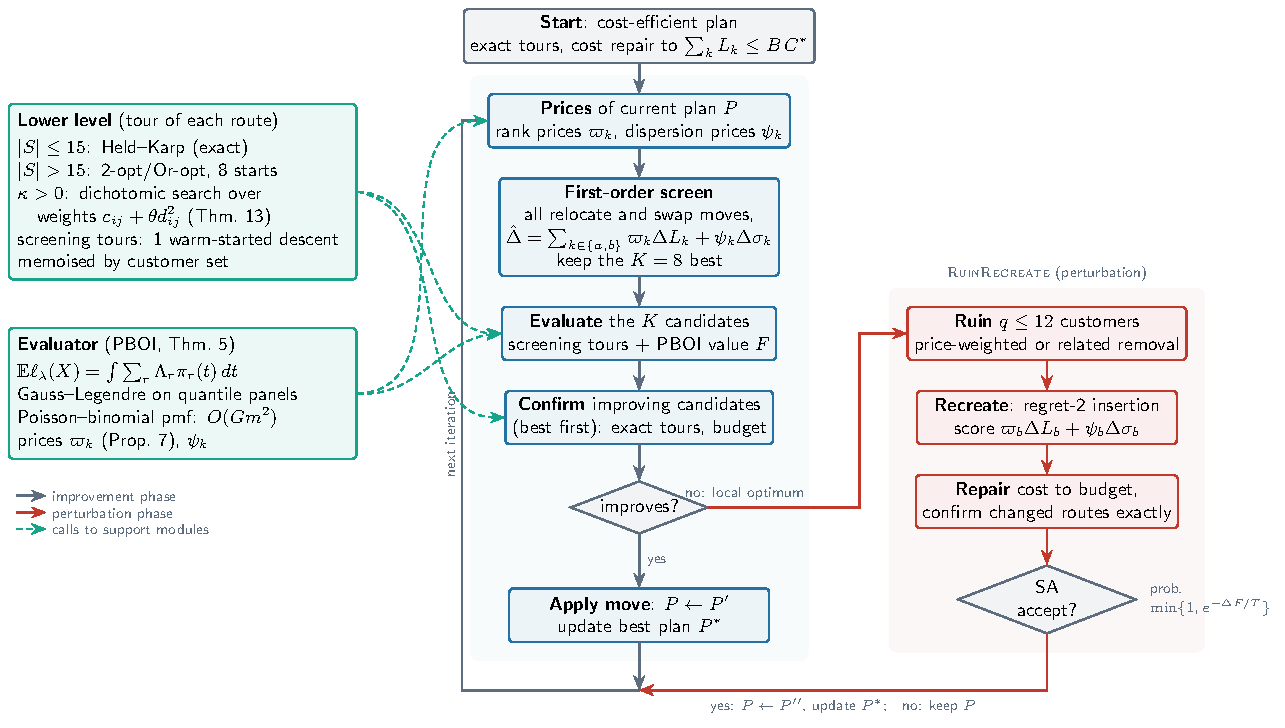
\includegraphics[width=\textwidth]{fig_algorithm.pdf}
\caption{The SORTIE algorithm. The improvement phase (blue) screens every
relocate and swap move with the rank and dispersion prices, evaluates the $K$
best with screening tours and PBOI, and confirms improving candidates with the
exact lower level. When no confirmed move improves the plan, the perturbation
phase (red) removes and reinserts customers guided by the same prices,
repairs the budget, confirms the changed routes and accepts by simulated
annealing. The two support modules (green) supply tours and objective values;
dashed arrows mark their calls.}\label{fig:algorithm}
\end{figure}

\begin{algorithm}[t]
\caption{SORTIE: main loop}\label{alg:sortie}
\begin{algorithmic}[1]
\Require instance, measure $\lambda$, noise level $v$, risk weight $\kappa$, budget $B\,C^\ast$, time limit
\State $P\gets$ cost-efficient plan; re-solve every route with the exact lower level; repair cost if $\sum_kL_k>B\,C^\ast$
\State $P^\ast\gets P$; $T_0\gets0.02\,|\E\lord(X(P))|$; \textit{stuck}$\gets$\textsc{none}
\While{time remains}
  \State compute rank prices $\varpi$ and dispersion prices $\psi$ of $P$ (Prop.~\ref{prop:prices})
  \If{\textit{stuck}$\neq P$}
    \State $P'\gets$\textsc{ImproveStep}$(P,\varpi,\psi)$ \Comment{screen, evaluate, confirm (\S\ref{sec:alg:screen}--\ref{sec:alg:confirm})}
    \If{$P'\neq$\textsc{none}} $P\gets P'$; update $P^\ast$; \textbf{continue}
    \Else\ \textit{stuck}$\gets P$
    \EndIf
  \EndIf
  \State $P''\gets$\textsc{RuinRecreate}$(P,\varpi,\psi)$; repair cost; confirm changed routes exactly
  \State accept $P''$ with probability $\min\{1,\exp(-(F(P'')-F(P))/T)\}$, $T=T_0\,(10^{-3})^{\,\text{elapsed}/\text{limit}}$
  \State update $P^\ast$
\EndWhile
\State \Return $P^\ast$
\end{algorithmic}
\end{algorithm}



\subsection{Representation and lower level}\label{sec:alg:lower}
A solution is a list of $m$ customer sequences, one per vehicle. The upper
level is the partition; the sequence of each route is not a decision of the
upper level but the output of the lower-level solver applied to the route's
customer set $S$. For $\kappa=0$ the lower level returns a shortest tour of
$\{0\}\cup S$, with ties broken by smaller quadratic length. For $|S|\le15$ it
is solved exactly by the Held--Karp recursion \citep{heldkarp1962dynamic}
compiled with numba, in $O(2^{|S|}|S|^2)$ time (about 5\,ms at 15
customers); for larger sets we use 2-opt and Or-opt (segments of one to three
customers, both orientations) from eight starts: a warm start built from the
route's previous sequence by cheapest insertion of new customers, the
nearest-neighbour tour, and random permutations. For $\kappa>0$ the lower
level minimises $\rho_\kappa=L+\kappa v\sqrt W$ by the dichotomic search of
Theorem~\ref{thm:supported}: starting from the tour minimising $L$ (ties by
$W$) and the tour minimising $W$ (ties by $L$), it repeatedly solves the
weighted problem with arc weights $c_{ij}+\theta d_{ij}^2$, where $\theta$ is
the slope between two known supported tours and $d_{ij}=H_{ij}c_{ij}$ (so
$d=c$ under homogeneous noise), until no new supported tour appears; every
weighted problem is solved like the $\kappa=0$ case. Lower-level results are
memoised by customer set, so a set that reappears during the search is never
solved twice.

\subsection{Evaluation}\label{sec:alg:eval}
Given the tour lengths $L_k$ and quadratic lengths $W_k$, every route has
mean $L_k$ and standard deviation $\sigma_k=v\sqrt{W_k}$, and its duration is
modelled by a gamma marginal with these two moments (normal marginals are an
option; E16 shows that the choice hardly matters). The objective
$F(P)=\E\lord(X)$ is evaluated by the integral of Theorem~\ref{thm:pboi}. The
integrand is smooth between the quantiles of the marginals and changes
quickly near them, so we integrate by six-point Gauss--Legendre rules on the
panels delimited by the quantiles of every marginal at 13 levels from
$10^{-12}$ to $1-10^{-12}$; with $m=5$ this gives about 360 nodes. At each node
the Poisson--binomial probability mass function of the number of routes
finished by time $t$ is computed by the standard recursion over routes in
$O(m^2)$, so one evaluation costs $O(Gm^2)$ for $G$ nodes, about $0.4$\,ms.
The rank prices of Proposition~\ref{prop:prices} reuse the same nodes, with
the mass function of the other $m-1$ routes, in $O(Gm^3)$; the dispersion
prices $\psi_k=\partial F/\partial\sigma_k$ are obtained by forward
differences with step $0.05\,\sigma_k$, i.e.\ $m$ further evaluations. For the
expected empirical variance all quantities are in closed form
(Proposition~\ref{prop:gap}). Prices are computed once per accepted plan.

\subsection{First-order screening}\label{sec:alg:screen}
The neighbourhood consists of all \emph{relocate} moves (customer $i$ from
route $a$ to route $b$) and all \emph{swap} moves (customers $i\in a$ and
$j\in b$ exchanged), about $n(m-1)+n^2(m-1)/(2m)$ moves in total. Evaluating
every move exactly would require two lower-level solves and one PBOI
evaluation per move. Instead, for every route we precompute, in vectorised
form, the change in $L$ and $W$ caused by removing each of its customers
(bridging its neighbours), by inserting any customer at its cheapest position,
and by replacing each of its customers by any other customer at the cheapest
position in the shortened route. These insertion deltas approximate the
change of the route statistics, and the change of the objective is predicted
to first order by the prices:
\begin{equation}\label{eq:pred}
\hat\Delta=\sum_{k\in\{a,b\}}\Big(\varpi_k\,\Delta L_k+\psi_k\,v\big(\sqrt{W_k+\Delta W_k}-\sqrt{W_k}\big)\Big).
\end{equation}
Moves that violate capacity, or whose predicted total length exceeds the
budget by more than $\epsilon_B=2\%$, are discarded; the remaining moves are
ranked by $\hat\Delta$ and the best $K=8$ are evaluated. By
Proposition~\ref{prop:prices}, $\varpi_k$ is the exact derivative of $F$
with respect to a shift of route $k$, so~\eqref{eq:pred} is the
linearisation of $F$ in the route statistics, with the insertion deltas
standing in for the re-optimised tours. A negative $\varpi_k$ (possible for the
range, the GMD and the MAD) predicts a gain from \emph{lengthening} route $k$,
which is exactly the incentive the lower level neutralises; the screen
therefore proposes such moves, and the exact evaluation then reveals whether
they survive the re-optimisation of the tour. E14 shows that the prediction
ranks moves with a Spearman correlation of about $0.9$ with their exact
effect. For the deterministic baseline the same screen is used with the
deterministic rank prices ($\lambda$ at the rank of each route, $\psi=0$),
for SAA with the empirical rank frequencies over the scenarios, and for
Det-$\sigma$ with the deterministic prices of $L+\sigma$, so all methods share
the search and differ only in the objective.

\subsection{Exact confirmation}\label{sec:alg:confirm}
The $K$ candidates are evaluated with \emph{screening tours}: a single
2-opt/Or-opt descent from the warm start (for $\kappa>0$ inside the same
dichotomic search, capped at 24 tours), without Held--Karp. Improving
candidates are then confirmed in order of their screened value: both changed
routes are re-solved by the exact lower level, the objective is re-evaluated,
and the move is applied only if it still improves and respects the budget.
Plans produced by the perturbation are confirmed route by route in the same
way.

\begin{proposition}[Bilevel feasibility of accepted plans]\label{prop:confirm}
Every plan that Algorithm~\ref{alg:sortie} accepts as its current or best plan
is capacity feasible, satisfies $\sum_kL_k\le B\,C^\ast$, and routes every
customer set on the tour returned by the exact lower level.
\end{proposition}
\begin{proof}
The start plan is re-solved by the exact lower level and repaired by cost
descent, whose steps are themselves confirmed moves. A plan becomes current
only through \textsc{ImproveStep}, which returns a plan only after re-solving
the two changed routes exactly and re-checking the budget, or through the
perturbation, whose output is accepted only after every route that differs
from the current plan has been re-solved exactly and the budget re-checked.
All other routes are unchanged and were exact before. Capacity is checked
for every move and every insertion.
\end{proof}

The screening tour is never shorter than the exact one, so a move that
improves only with exact tours can be missed; this affects the quality of the
search, not feasibility. E14 shows that 28 of 30 final SORTIE plans admit no
improving relocate or swap move at all, i.e.\ the search ends in genuine
local optima of the neighbourhood. Together with a cap on the ruin size, lazy
confirmation raises the iteration rate of SORTIE-0 at $n=100$ from about 250
to about 1700 per minute, and at $n=75$ from about 170 to about 1800.

\subsection{Perturbation and acceptance}\label{sec:alg:perturb}
When no screened move improves the current plan, SORTIE applies a
ruin-and-recreate perturbation. The number of removed customers $q$ is drawn
uniformly from $\{2,\dots,\max(3,\min(12,\lceil n/4\rceil))\}$. With
probability $1/2$ the removal pool is \emph{price-weighted}: routes are
ordered by sampling without replacement with probabilities proportional to
$|\varpi_k|$, and their customers are added to the pool until it holds at
least $q$; otherwise the pool is all customers. From the pool, with
probability $1/2$ the $q$ customers closest to a random seed customer are
removed (related removal), otherwise $q$ random customers; no route is
emptied. The removed customers are reinserted by \emph{price-scored regret-2
insertion}: inserting customer $i$ at its cheapest position in route $b$ is
scored by
\[
s_b(i)=\varpi_b\,\Delta L_b+\psi_b\,\Delta\sigma_b+10^{-3}\,\Delta L_b,
\]
the customer with the largest difference between its best and second-best
capacity-feasible score is inserted first, and the scores of the modified
route are updated. The small cost term breaks ties in favour of shorter
insertions. If the result exceeds the budget it is repaired by cost descent:
\textsc{ImproveStep} with unit prices and zero dispersion prices, so that
$\hat\Delta$ is the change in total length, for at most 200 steps; if the
budget cannot be met the perturbation is discarded. The repaired plan is
confirmed exactly (\S\ref{sec:alg:confirm}) and accepted by simulated
annealing with temperature $T=T_0(10^{-3})^{\tau}$, where $\tau$ is the
elapsed fraction of the time limit. The initial temperature
$T_0=0.02\,|\E\lord(X(P_0))|$ is computed from the PBOI value of the start
plan for every method, so that Det, SAA and SORTIE accept uphill moves of the
same absolute size.

\subsection{Parameters and complexity}\label{sec:alg:params}
The parameters (listed in the Online Supplement) are the same for all methods and instances; none was tuned per instance.
E14 shows that the number of evaluated candidates $K$ between 1 and 32 does not
change the median result. One improvement step costs the precomputation of
the deltas, $O(m\,n_k^2N)$ for routes of $n_k$ customers and $N=n+1$ nodes,
which is vectorised; the ranking of all moves, $O(n^2)$; $K$ screening
re-solves of two routes, each a local-search descent; $K$ PBOI evaluations,
$O(KGm^2)$; and at most a few exact re-solves. The prices cost
$O(Gm^3)+m$ PBOI evaluations per accepted plan. On the main grid an iteration takes 7 to 9\,ms (median), and the search
runs 2300 to 3100 iterations in 15 to 25\,s; at $n=100$ it runs about 3500
iterations in 120\,s (E7).



%==========================================================================

\section{Computational study}\label{sec:exp}

This section reports the main experiments; the Online Supplement contains
further analyses (rank-price diagnostics, noise level, fleet size, day-factor
dispersion, drivers' risk attitude, congestion and per-instance results), to
which we refer by their labels E1--E17. All code, instances, solved plans and
raw results are released (see the data availability statement), and every
table and figure is generated from the raw results by the released scripts.

\subsection{Set-up}\label{sec:exp:setup}
\paragraph{Instances.} We follow the slicing rule of the deterministic fair
routing literature \citep{ljubic2026fair}. Block $b$ of size $n$ consists of the
depot and the $n$ consecutive customers $bn+1,\dots,(b+1)n$ of the CVRPLIB
instance X-n641-k35 \citep{uchoa2017new}, with ceiled Euclidean distances,
$m=5$ vehicles and capacity $Q=\lfloor\sum_iq_i/4\rfloor$, so that one
vehicle's worth of slack is available. The main grid uses
$n\in\{15,20,25,30,35\}$ and blocks $b=0,\dots,4$ (25 instances); the scale
test uses $n\in\{50,75,100\}$ with six blocks each. A second family takes the
depot and the first 50 customers of twelve further X instances (X-n101-k25 to
X-n153-k22), which keeps their original depot positions and customer
distributions (Section~\ref{sec:exp:family}).

\paragraph{Uncertainty and budget.} Unless stated otherwise the arc noise has
coefficient of variation $v=0.3$ (gamma) and the day factor $s_Y=0.15$.
$C^\ast$ is the cost of the best of three restarts of the cost-minimising
search, and the total length of every fair plan must satisfy
$\sum_kL_k\le B\,C^\ast$ with $B=1.10$ unless stated otherwise.

\paragraph{Methods.} All methods use the search of Section~\ref{sec:alg} with
the same start plan, random seed and time limit (15\,s for $n\le25$, 25\,s for
$n\in\{30,35\}$, 120\,s for $n\ge50$); they differ only in the objective and its
prices. \emph{Det} minimises the deterministic measure $\lord(L)$, i.e.\ the
model of \citet{ljubic2026fair} solved heuristically. \emph{SAA} minimises the
sample average of $\lord(X)$ over 200 fixed scenarios. \emph{Det-$\sigma$}
minimises the deterministic measure of the risk-adjusted lengths $L_k+\sigma_k$.
\emph{SORTIE-0} minimises the exact ex-post value with shortest tours
($\kappa=0$) and \emph{SORTIE-1} with risk-consistent tours ($\kappa=1$).

\paragraph{Evaluation.} Every plan is evaluated out of sample by arc-level
Monte Carlo simulation with $20\,000$ scenarios ($10\,000$ for $n\ge 50$),
including the day factor, with common random numbers across methods. The
reported \emph{ex-post value} is the simulated $\E\lord(\Phi)$; improvements are
relative to Det, and paired comparisons use the Wilcoxon signed-rank test.

\subsection{Accuracy of the evaluator}\label{sec:exp:accuracy}
Table~\ref{tab:e1} compares PBOI with $50\,000$-scenario arc-level simulation
on 168 plans (cost-efficient and random feasible plans, $n\in\{15,25,35,50\}$).
The mean absolute relative error is at most $0.11\%$ for every measure and the
worst case $0.44\%$; the small systematic bias (mean $z$-scores up to $0.34$)
comes from the moment-matched gamma marginals. PBOI takes $0.44$\,ms per plan
for $m=5$, against $0.28$\,s for $20\,000$-scenario simulation; a 200-scenario
sample average is faster ($0.06$\,ms) but noisy. On ten instances with $n=10$
and $m=3$ we also enumerated every capacity- and budget-feasible partition
with exact tours: SORTIE-0 found the plan with the smallest exact ex-post value
on nine of ten instances (mean gap $0.39\%$, maximum $3.9\%$).

\begin{table}[t]\centering\small
\caption{Accuracy of PBOI against arc-level simulation ($50\,000$ scenarios)
on 168 plans; $z$: difference over its simulation standard error.}\label{tab:e1}
\begin{tabular}{lrrrr}\toprule
Measure & Plans & Mean $|$err$|$ (\%) & Max $|$err$|$ (\%) & Share $|z|<3$ \\
\midrule
Max & 168 & 0.041 & 0.137 & 0.994 \\
Range & 168 & 0.062 & 0.249 & 1.000 \\
GMD & 168 & 0.057 & 0.241 & 1.000 \\
MAD & 168 & 0.064 & 0.272 & 0.988 \\
Var & 168 & 0.108 & 0.440 & 0.994 \\
\bottomrule
\end{tabular}

\end{table}

\subsection{The fairness illusion and the value of ex-post optimisation}\label{sec:exp:main}
Table~\ref{tab:illusion} quantifies Propositions~\ref{prop:gap}
and~\ref{prop:balance}. The value a deterministic fair plan reports understates
the true ex-post value by $8\%$ for the maximum, $15$--$18\%$ for the range, GMD
and MAD, and $27\%$ for the variance. The in-sample SAA value is optimistic by
about $1\%$ (the optimiser's curse), and the PBOI value believed by SORTIE has a
mean signed error below $0.1\%$. In line with Proposition~\ref{prop:balance},
the cost-optimal plans, whose routes are far from balanced, are misjudged by
only $4$--$6\%$.

\begin{table}[t]\centering\small
\caption{Believed against true ex-post value (mean signed \%, 50 runs per
cell; truth: simulation without the day factor, which is what each model
represents). Last column: largest absolute PBOI error for any plan.}\label{tab:illusion}
\begin{tabular}{lrrrrr}\toprule
 & \multicolumn{4}{c}{Believed vs true (mean signed \%)} & PBOI \\
Measure & Det & SAA & SORTIE-0 & SORTIE-1 & max $|$err$|$ \% \\
\midrule
Max & -7.97 & -0.71 & -0.01 & -0.01 & 0.20 \\
Range & -17.56 & -0.99 & +0.03 & +0.02 & 0.70 \\
GMD & -14.68 & -0.91 & +0.04 & +0.05 & 0.61 \\
MAD & -16.17 & -0.88 & +0.05 & +0.07 & 0.68 \\
Var & -27.23 & -1.33 & +0.00 & +0.02 & 0.98 \\
\bottomrule
\end{tabular}

\end{table}

Table~\ref{tab:e3} reports the out-of-sample ex-post value relative to Det on
the 25 instances, five measures and two budgets. Pooled over the 250 runs,
SORTIE-0 improves on Det by $0.89\%$ on average (median $0.23\%$; better in 141
runs, tied in 96, worse in 13; $p<10^{-18}$) and SORTIE-1 by $0.77\%$ (better in
154, worse in 31). SAA improves by only $0.14\%$ (better in 115, worse in 74),
and both SORTIE variants beat it head to head ($p<10^{-17}$). The largest gain
is for the maximum at $B=1.10$ ($2.1\%$, 24 of 25 instances). The gains are
modest because under homogeneous noise a route's standard deviation grows with
its length, so balancing lengths roughly balances risks: the deterministic
plan's \emph{choice} is often close to the best one, while its
\emph{assessment} of its own fairness is badly wrong. For context, the
cost-optimal plan has an expected realised range of 2087 against about 1340 for
the fair plans, at a $6.5\%$ higher cost.

\begin{table}[t]\centering\small
\caption{Improvement of the out-of-sample ex-post value over Det (mean \%,
positive is better; in brackets the number of instances, of 25, on which the
method is strictly better). $^\ast$: Wilcoxon signed-rank $p<0.05$ in favour
of the method.}\label{tab:e3}
\begin{tabular}{llrrr}\toprule
Measure & $B$ & SAA & SORTIE-0 & SORTIE-1 \\
\midrule
GMD & 1.05 & -0.40 (6/25) & -0.09 (8/25) & -0.03 (9/25) \\
GMD & 1.10 & -0.32 (9/25) & +0.94$^\ast$ (14/25) & +0.34$^\ast$ (17/25) \\
MAD & 1.05 & +0.86$^\ast$ (11/25) & +1.10$^\ast$ (13/25) & +1.24$^\ast$ (12/25) \\
MAD & 1.10 & +0.70 (13/25) & +0.96$^\ast$ (14/25) & +1.53$^\ast$ (18/25) \\
Max & 1.05 & +0.71$^\ast$ (14/25) & +0.61$^\ast$ (15/25) & +0.77$^\ast$ (15/25) \\
Max & 1.10 & +1.70$^\ast$ (23/25) & +2.08$^\ast$ (24/25) & +1.93$^\ast$ (24/25) \\
Range & 1.05 & +0.12 (13/25) & +0.64$^\ast$ (15/25) & +1.56$^\ast$ (15/25) \\
Range & 1.10 & -0.21 (13/25) & +1.07$^\ast$ (17/25) & +0.39$^\ast$ (15/25) \\
Var & 1.05 & +0.48 (7/25) & +0.50$^\ast$ (9/25) & +0.48$^\ast$ (13/25) \\
Var & 1.10 & -2.25 (6/25) & +1.09$^\ast$ (12/25) & -0.49$^\ast$ (16/25) \\
\bottomrule
\end{tabular}

\end{table}

Figure~\ref{fig:workloads} shows what the drivers of a representative instance
(X641-n30-b0, whose SORTIE-0 gain is close to the median) experience. The
realised workloads are wide and right-skewed, and the expected realised range
of both fair plans is about 1225, $30\%$ above the deterministic range of about
940 that the Det planner reports.

\begin{figure}[t]\centering
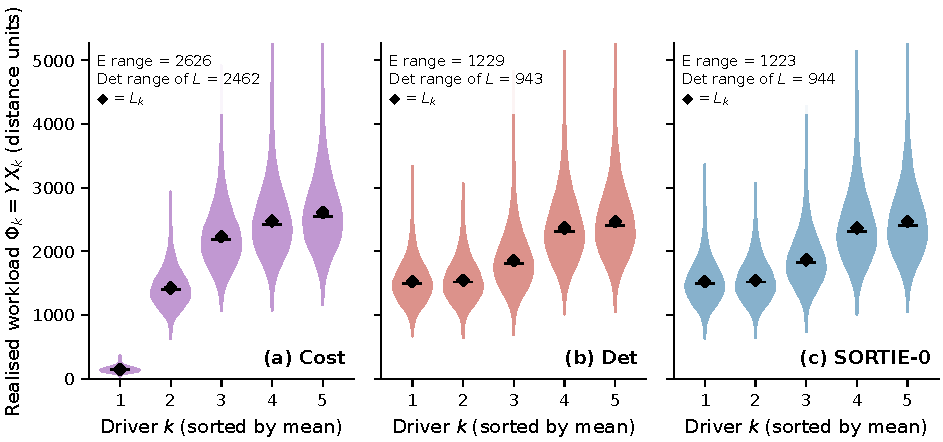
\includegraphics[width=\textwidth]{fig_workloads.pdf}
\caption{Simulated realised workloads $\Phi_k=YX_k$ of the cost-optimal,
Det and SORTIE-0 range plans of X641-n30-b0 ($20\,000$ days); diamonds mark the
tour lengths seen by a deterministic model.}\label{fig:workloads}
\end{figure}

\paragraph{Route consistency.} Without the lower level, i.e.\ letting the
planner sequence each route freely, 23 of 25 Det plans and 24 of 25 SORTIE
plans for the range contain a route that is not a shortest tour of its
customers, with an average excess length of 95 and 113 distance units. These
detours lower the measured unfairness by $1$--$3\%$, and they are exactly the
behaviour signalled by negative rank prices and excluded by the bilevel
constraint (E4 in the Online Supplement).

\subsection{The budget frontier}\label{sec:exp:budget}
Figure~\ref{fig:frontier} varies the budget factor from $B=1.02$ to $1.30$ on
the ten instances with $n\in\{25,35\}$. The gain of SORTIE-0 over Det grows
with the budget, from about $1\%$ for $B\le1.10$ to $3.2\%$ at $B=1.15$ and
$6.8\%$ at $B=1.30$, where SORTIE-0 is better on all 30 instance--measure pairs.
With little slack every fair plan is close to the cost-optimal one; with more
slack many plans have about the same deterministic range but different
realised ranges, and only the ex-post objective can tell them apart. For
$B\ge1.15$ SORTIE-0 also uses \emph{less} of the budget: at $B=1.30$ the Det
plans for the maximum have a total length $20.5\%$ above $C^\ast$ and an
expected realised maximum $5.2\%$ below that of the cost plan, whereas the
SORTIE-0 plans use $13.5\%$ and achieve $8.7\%$. The deterministic objective
spends extra length on routes whose deterministic length is irrelevant to the
maximum but whose variance raises the realised one.

\begin{figure}[t]\centering
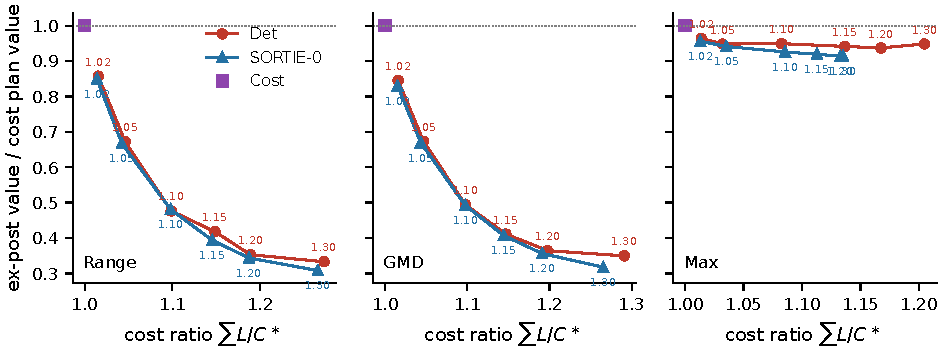
\includegraphics[width=\textwidth]{fig_e9_frontier.pdf}
\caption{Price of fairness: mean total length relative to $C^\ast$ against the
mean expected realised unfairness relative to the cost-optimal plan, for budget
factors $B$ from 1.02 to 1.30 (labels), $n\in\{25,35\}$.}\label{fig:frontier}
\end{figure}

\subsection{Simpler alternatives}\label{sec:exp:baselines}
Two natural alternatives to the exact integral are a larger sample and a
risk-adjusted deterministic model (Table~\ref{tab:baselines}). SORTIE-0 is
better than SAA with $S\in\{50,200,1000,5000\}$ scenarios by $1.4$, $1.6$,
$1.1$ and $0.9\%$, significantly for $S\le1000$; at $S=5000$ SAA is still worse
on 9 pairs and better on 2 of 30, but no longer significantly ($p=0.05$).
Det-$\sigma$, which balances $L_k+\sigma_k$, is \emph{worse} than Det
($-0.8\%$, better on 37 and worse on 61 of 125 pairs, $p=0.02$), and SORTIE-0
beats it by $1.9\%$ (97 of 125 pairs). Adding a safety margin to every route
treats each route's risk separately, whereas the expected ordered measure
depends on how likely each route is to occupy each rank, which is what the
Poisson--binomial integral and the rank prices capture. Replacing the gamma
marginals of PBOI by normal ones changes nothing significant ($p=0.65$).

\begin{table}[t]\centering\small
\caption{Simpler alternatives, $B=1.10$: improvement over Det of the
risk-adjusted model (Det-$\sigma$), of PBOI with normal marginals (PBOI-N) and
of SORTIE-0 on the 25 main-grid instances (format as Table~\ref{tab:e3}; the
variance is omitted for PBOI-N, whose value does not depend on the marginal
family for that measure).}\label{tab:baselines}
\begin{tabular}{lcccc}
\toprule
Measure & Det-$\sigma$ vs Det & PBOI-N vs Det & SORTIE-0 vs Det & SORTIE-0 vs Det-$\sigma$ \\
\midrule
Range & -0.49 (8/25) & +0.48$^\ast$ (18/25) & +1.07$^\ast$ (17/25) & +1.51$^\ast$ (19/25) \\
GMD & -0.69 (8/25) & +0.83$^\ast$ (14/25) & +0.94$^\ast$ (14/25) & +1.50$^\ast$ (18/25) \\
Max & -0.08 (8/25) & +2.08$^\ast$ (24/25) & +2.08$^\ast$ (24/25) & +2.13$^\ast$ (25/25) \\
Pooled & -0.81$^\dagger$ (37/125) & +1.10$^\ast$ (71/100) & +1.23$^\ast$ (81/125) & +1.86$^\ast$ (97/125) \\
\bottomrule
\end{tabular}

\end{table}

\subsection{A second benchmark family}\label{sec:exp:family}
All instances so far are slices of one file, and slicing places the depot at
the first node of each block. We therefore solved the depot and the first 50
customers of twelve further CVRPLIB X instances \citep{uchoa2017new}, which
were generated with different depot positions and customer distributions,
with $m=5$, the same capacity rule, $B=1.10$, 120\,s and two solver seeds
(Table~\ref{tab:e17}). The illusion reaches $40\%$ for the range and $35\%$ for
the GMD, against $23\%$ and $19\%$ on the sliced instances at the same budget.
SORTIE-0 improves on Det by $2.2\%$ on average (median $1.7\%$; better on 31
and worse on 5 of 36 pairs, $p<10^{-6}$), with a positive average on every one
of the twelve instances ($0.7$ to $4.2\%$); SAA improves by $0.7\%$, and
SORTIE-0 beats it on 33 of 36 pairs.

\begin{table}[t]\centering\small
\caption{Second benchmark family (twelve X instances, depot and first 50
customers), $B=1.10$, mean of two solver seeds: improvement of the ex-post value
over Det (format as Table~\ref{tab:e3}).}\label{tab:e17}
\begin{tabular}{lcccc}
\toprule
Measure & SAA vs Det & SORTIE-0 vs Det & Det-$\sigma$ vs Det & Det belief err. (\%) \\
\midrule
Range & +1.48 (8/12) & +2.91$^\ast$ (11/12) & -0.39 (5/12) & -40.3 \\
GMD & -0.62 (5/12) & +1.64 (8/12) & -2.15$^\dagger$ (1/12) & -34.7 \\
Max & +1.36$^\ast$ (10/12) & +1.93$^\ast$ (12/12) & +0.01 (7/12) & -8.4 \\
Pooled & +0.74$^\ast$ (23/36) & +2.16$^\ast$ (31/36) & -0.84 (13/36) & -27.8 \\
\bottomrule
\end{tabular}

\end{table}

\subsection{Robustness and scale}\label{sec:exp:robust}
\emph{Noise model.} Re-evaluating the plans under lognormal, incident-type
(an arc takes 2.5 times as long with probability 0.02) and spatially
correlated noise with the same per-arc mean and variance raises the mean
absolute PBOI error from $0.16\%$ to $0.29$, $1.4$ and $1.9\%$ respectively,
but SORTIE-0 remains significantly better than Det under every family ($1.0$
to $1.2\%$). \emph{Congestion.} With a noise multiplier between $1/3$ and $2$
that is largest near a congestion centre, the illusion for the range grows
from $23\%$ to $26\%$ and the gain of SORTIE-0 to $1.5\%$ (53 of 75 pairs better,
3 worse). \emph{Fleet size and noise level.} The gain grows with the number of
vehicles ($3.2\%$ with seven vehicles) and with the noise level ($2.1\%$ for the
range at $v=0.5$). \emph{Size.} At $n=100$ single runs are dominated by search
noise; averaging three solver seeds of 240\,s, SORTIE-0 improves on Det by
$4.2\%$ (13 of 18 instance--measure pairs, $p=0.02$), while the difference from
SAA ($1.1\%$) is not significant. Strikingly, the Det plans for the range vary
by $11\%$ across seeds, against $3\%$ for SORTIE-0: the deterministic range is
flat over many plans whose realised fairness differs. Details are in
experiments E6--E8, E10 and E12 of the Online Supplement.

\subsection{Managerial insights}\label{sec:insights}
\emph{(i) Report realised, not planned, fairness.} A deterministic fair plan
understates the unfairness its drivers will experience, by more the more
balanced the plan; PBOI computes the realised value in under a millisecond for
any plan, whatever method produced it.
\emph{(ii) Do not spend the budget on deterministic balance.} With generous
budgets a deterministic fair model spends the slack on equalising route
lengths, which does little for realised fairness; the ex-post objective
achieves more with less.
\emph{(iii) Neither safety margins nor more scenarios are a substitute.}
Balancing risk-adjusted lengths is worse than ignoring uncertainty, and a
sample average needs thousands of scenarios to approach the exact objective.
\emph{(iv) Keep the shortest-tour requirement.} Without it, fairness is
bought with detours; under uncertainty it must be imposed explicitly, and the
risk-consistent variant changes few tours in practice (E13).

\section{Conclusions}\label{sec:concl}
Fair routing under random travel times has to say whose fairness it measures.
Drivers experience realised durations, so the relevant quantity is the
expected unfairness of the realised day. A deterministic fair plan cannot see
this quantity: in our experiments it understated it by $8$ to $27\%$ on the
sliced benchmark instances and by up to $40\%$ on a second instance family, and
Proposition~\ref{prop:balance} shows why the understatement is largest for the
balanced plans that fairness optimisation produces. Fleet-wide shocks, by
contrast, leave the expected value of every ordered measure unchanged, although
they inflate the tail of unfairness.

The Poisson--binomial order-statistic integral evaluates any ordered measure of
independent route durations exactly, in under a millisecond for five vehicles,
and its derivatives, the rank prices, are both interpretable and useful: they
identify the routes a fairness objective would like to lengthen, and they rank
candidate moves with a Spearman correlation of about $0.9$ with their exact
effect. Under uncertainty route consistency no longer follows from
monotonicity, so it has to be part of the model; the mean--standard-deviation
lower level makes it computable by parametric Held--Karp.

The improvement of the plan itself is significant but modest at the standard
budget, and it grows where the deterministic model has most freedom to choose
wrongly: with more slack in the budget (up to $7\%$, with a lower total
length), with more vehicles and on instances whose depot is not a block corner
($2.2\%$, better on all twelve instances of the second family). It survives
misspecified and spatially correlated noise, it is not reproduced by a
risk-adjusted deterministic model, and a sample average needs thousands of
scenarios to come close.

\paragraph{Limitations and future work.} The lower level is exact only for
routes of up to 15 customers; beyond that it relies on multi-start local
search, and the bilevel constraint is then satisfied only approximately. PBOI
assumes conditionally independent route durations; correlated congestion
reduces its accuracy (to about $2\%$ in our tests) although not the ranking of
plans. At 100 customers single runs are noisy, the risk-consistent variant is
too slow to converge, and SORTIE could not be separated statistically from a
200-scenario sample average. Exact methods for the stochastic bilevel problem
(branch-and-cut with PBOI-based bounds), correlated route durations, multi-day
fairness, in which unfairness can be compensated across days, and
time-dependent travel times are natural next steps.

\section*{Declaration of competing interest}
The authors declare that they have no known competing financial interests or
personal relationships that could have appeared to influence the work reported
in this paper.

\section*{Funding}
This research did not receive any specific grant from funding agencies in the
public, commercial, or not-for-profit sectors.

\section*{CRediT authorship contribution statement}
\textbf{Quang-Vinh Dang:} Conceptualization, Methodology, Formal analysis,
Software, Writing -- original draft, Supervision.
\textbf{Hoang-Viet Vu:} Software, Investigation, Validation, Visualization,
Writing -- review \& editing.
\textbf{Phuc-Son Nguyen:} Formal analysis, Validation, Writing -- review \&
editing.

\section*{Data availability}
The instances (CVRPLIB X instances), the code, all solved plans, the raw
results and the scripts that generate every table and figure will be made
publicly available in a repository upon acceptance and are available from the
corresponding author on request.

\section*{Declaration of generative AI and AI-assisted technologies in the manuscript preparation process}
During the preparation of this work the authors used Claude (Anthropic) to
support writing. After using this tool, the authors reviewed and edited the
content as needed and take full responsibility for the content of the
published article.

\bibliographystyle{apacite}
\bibliography{references}
\end{document}
